\chapter{نظرية مجال الربائط واللون}\label{ch:b2:ligand-field}

الياقوت أحمر والزمرد أخضر، ومع ذلك يدين كلاهما بلونه للأيون نفسه،
\ce{Cr^3+}، الذي يحل قليل منه محل الألومنيوم في الكوراندوم، \ce{Al2O3}، أو في
البيريل. وبلورات كبريتات النحاس زرقاء داكنة، لكن المسحوق المتبقي بعد
تسخينها أبيض. وفي كل حالة يأتي اللون من إلكترونات تقفز
بين مدارات d باعدت الذراتُ المحيطة بين طاقاتها ---
بمقدار يتوقف على الذرات المحيطة بالأيون وعلى كيفية إحاطتها به. ويحسب هذا
الفصل ذلك الانشطار، أولًا بشحنات نقطية، ثم \omterm{def:b2:diatomic-mos:lcao}{بالمدارات
الجزيئية}؛ ويفسر الألوان، والمغناطيسية، \omterm{def:b2:coordination-complexes:electron-count}{وقاعدة الثمانية عشر إلكترونًا} في
الفصل السابق.

\begin{recall}
\Cref{ch:b2:coordination-complexes}: توزيعات $d^n$، والهندسات، وعدّ
الإلكترونات. و\cref{ch:b2:atomic-orbitals}: أشكال مدارات d الخمسة.
و\cref{ch:b2:fragment-orbitals}: \omterm{def:b2:fragment-orbitals:fragment}{مدارات الشظايا}. ومجلد السنة الأولى: الامتصاصية،
والألوان المتتامة، والإلكترونات المنفردة، وقاعدة هوند.
\end{recall}

\begin{omfigure}
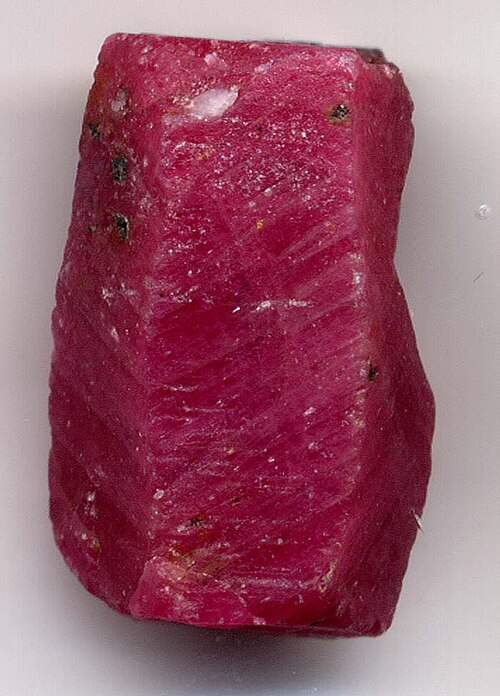
\includegraphics[height=3.6cm]{images/book3/ruby.jpg}\hspace{0.6cm}%
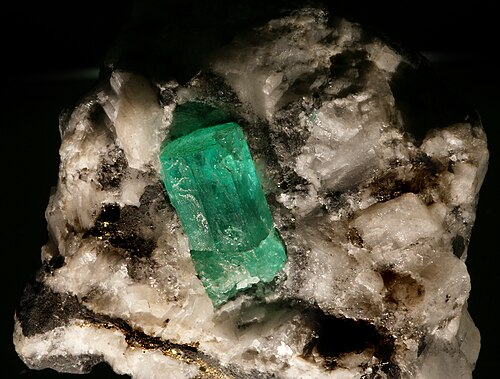
\includegraphics[height=3.6cm]{images/book3/emerald.jpg}\hspace{0.6cm}%
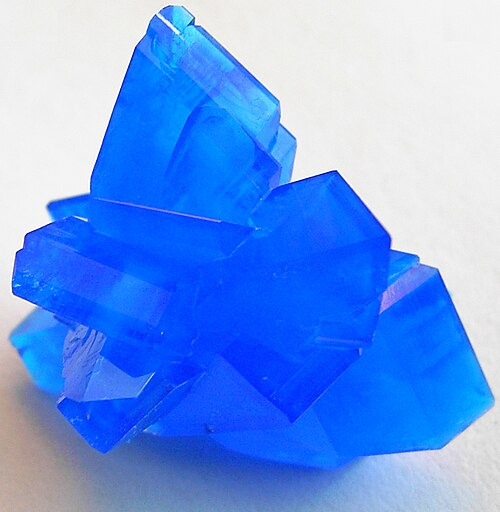
\includegraphics[height=3.6cm]{images/book3/copper-sulfate.jpg}

{\small بلورة ياقوت (ملكية عامة)؛ وزمردة في صخرتها (ديدييه ديكوان،
CC~BY-SA~3.0)؛ وبلورات كبريتات النحاس(II) الخماسية الماء (ستيفانب، CC~BY-SA~3.0)،
ويكيميديا كومنز. والكروم(III) هو ما يلوّن الأوليين، والمعقد المائي
للنحاس(II) هو ما يلوّن الثالثة.}
\end{omfigure}

\section{نموذج المجال البلوري}

\begin{definition}[المجال البلوري]\label{def:b2:ligand-field:crystal-field}
\emph{نموذج المجال البلوري}\index{نموذج المجال البلوري} يعامل ربائط
المعقد على أنها شحنات نقطية سالبة (أو أطراف سالبة لثنائيات أقطاب) حول أيون
الفلز، ويحسب كيف تغيّر طاقات مداراته d. وفي مجال
ثماني الأوجه، تنشطر مدارات d إلى مجموعتين يفصل بينهما \emph{انشطار المجال
البلوري}\index{انشطار المجال البلوري} $\Delta_o$.
\end{definition}

ضع الربائط الست على المحاور. يوجّه المداران $\mathrm d_{z^2}$ و$\mathrm d_{x^2-y^2}$
فصوصهما مباشرة نحو الربائط: فيتنافر الإلكترون فيهما أكثر
ويرتفعان. أما المدارات $\mathrm d_{xy}$ و$\mathrm d_{xz}$ و$\mathrm d_{yz}$ فتتجه بين
الربائط وترتفع أقل. ويسمى الزوج الأول $e_g$، والمجموعة الثانية الثلاثية
$t_{2g}$ (أسماء من نظرية الزمر، في مجلد السنة الثالثة).

\begin{omfigure}
\begin{tikzpicture}[font=\small]
  \begin{scope}
    \pic at (0,0) {omdx2y2};
    \foreach \p in {(1.25,0),(-1.25,0),(0,1.25),(0,-1.25)} \node[circle, fill=black!70, inner sep=2.2pt] at \p {};
    \node at (0,-1.75) {\foreignlanguage{arabic}{$\mathrm d_{x^2-y^2}$: فصوص نحو الربائط}};
  \end{scope}
  \begin{scope}[xshift=5.5cm]
    \pic at (0,0) {omdxy};
    \foreach \p in {(1.25,0),(-1.25,0),(0,1.25),(0,-1.25)} \node[circle, fill=black!70, inner sep=2.2pt] at \p {};
    \node at (0,-1.75) {\foreignlanguage{arabic}{$\mathrm d_{xy}$: فصوص بينها}};
  \end{scope}
\end{tikzpicture}

{\small مداران من مدارات d بين الربائط الأربع للمستوي $xy$ في ثماني أوجه
(النقاط السوداء). تتجه فصوص $\mathrm d_{x^2-y^2}$ نحو الربائط، وفصوص
$\mathrm d_{xy}$ بينها.}
\end{omfigure}

\begin{theorem}[مركز الثقل]\label{thm:b2:ligand-field:barycentre}
في مجال ثماني الأوجه، وبالقياس من متوسط طاقة مدارات d، يقع
الزوج $e_g$ عند $+0.6\Delta_o$ والمجموعة $t_{2g}$ عند $-0.4\Delta_o$.
\end{theorem}

\begin{proof}
يرفع المجال متوسط طاقات d الخمس لكنه لا يغيّره
بالانشطار (قاعدة مركز الثقل، مقبولة: مجموع انزياحات مجموعة كاملة من
المدارات تحدده الشحنة الكلية، لا ترتيبها). ومع $e_g$ عند $x$ 
و$t_{2g}$ عند $x - \Delta_o$، يعطي الشرط $2x + 3(x - \Delta_o) = 0$ القيمة $x = 0.6\Delta_o$.
\end{proof}

\section{السبين المرتفع والسبين المنخفض}

\begin{definition}[حالات السبين]\label{def:b2:ligand-field:spin}
\emph{طاقة الاقتران}\index{طاقة الاقتران} $P$ هي الطاقة اللازمة لوضع إلكترون ثانٍ
في مدار مشغول بدلًا من مدار فارغ له الطاقة نفسها. ويكون
المعقد \emph{عالي السبين}\index{عالي السبين} حين تشغل إلكتروناته مداري $e_g$
قبل أن تقترن في $t_{2g}$، و\emph{منخفض السبين}\index{منخفض السبين} حين تقترن في $t_{2g}$
أولًا.
\end{definition}

\begin{proposition}[اختيار حالة السبين]\label{prop:b2:ligand-field:spin-state}
من أجل الأيونات الثمانية الأوجه من $d^4$ إلى $d^7$، يكون المعقد \omterm{def:b2:ligand-field:spin}{منخفض السبين} إذا كان $\Delta_o > P$ \omterm{def:b2:ligand-field:spin}{وعالي السبين}
إذا كان $\Delta_o < P$. ومن أجل $d^1$--$d^3$ و$d^8$--$d^{10}$ لا يوجد إلا توزيع واحد.
\end{proposition}

\begin{proof}
انطلاقًا من $d^3$ ($t_{2g}^3$)، فإن الإلكترون الرابع إما يدخل $e_g$ (الكلفة $\Delta_o$ فوق
$t_{2g}$) وإما يقترن في $t_{2g}$ (الكلفة $P$). فيغلب الأرخص؛ وتصح المقارنة نفسها
لكل إلكترون حتى $d^7$. ومن أجل $d^1$--$d^3$ يتسع $t_{2g}$ دون اقتران؛
ومن أجل $d^8$--$d^{10}$، يكون $t_{2g}$ ممتلئًا ولا بد من استعمال $e_g$ على أي حال.
\end{proof}

\begin{definition}[طاقة استقرار المجال البلوري]\label{def:b2:ligand-field:cfse}
\emph{طاقة استقرار المجال البلوري}\index{طاقة استقرار المجال البلوري}
(CFSE) لتوزيع $t_{2g}^ae_g^b$ هي $(-0.4a + 0.6b)\Delta_o$، أي طاقة
إلكترونات d بالنسبة إلى مركز الثقل (وطاقات الاقتران تُحسب على حدة).
\end{definition}

\begin{proposition}[طاقة استقرار المجال البلوري على طول السلسلة]\label{prop:b2:ligand-field:cfse}
في حالة السبين المرتفع، تكون CFSE مساوية $0$، $-0.4$، $-0.8$، $-1.2$، $-0.6$، $0$، $-0.4$، $-0.8$، $-1.2$،
$-0.6$، $0$ (بوحدة $\Delta_o$) من أجل $d^0$ إلى $d^{10}$: فتنعدم من أجل $d^0$، $d^5$، $d^{10}$. وفي حالة السبين
المنخفض تبلغ $-2.4\Delta_o$ من أجل $d^6$.
\end{proposition}

\begin{proof}
املأ التوزيعات وطبّق التعريف؛ والقيم هي قيم الشكل،
محسوبة.
\end{proof}

\begin{omfigure}
\begin{tikzpicture}
\begin{axis}[width=0.55\linewidth, height=5cm, xmin=-0.5, xmax=10.5, ymin=-2.6, ymax=0.3,
  axis x line=bottom, axis y line=left, xlabel={$d^n$}, ylabel={\babelsublr{CFSE ($\Delta_o$)}},
  xtick={0,1,2,3,4,5,6,7,8,9,10}, tick label style={font=\small}, label style={font=\small}]
\addplot[omThm, thick, mark=*, mark size=1.3pt] table[x=n, y=high] {figdata/out/bachelor-2-ligand-field-a.dat};
\addplot[omDef, thick, dashed, mark=square*, mark size=1.3pt] table[x=n, y=low] {figdata/out/bachelor-2-ligand-field-a.dat};
\node[font=\scriptsize, omThm, anchor=west] at (axis cs:5.4,0.0) {\foreignlanguage{arabic}{سبين مرتفع}};
\node[font=\scriptsize, omDef, anchor=west] at (axis cs:6.6,-2.2) {\foreignlanguage{arabic}{سبين منخفض}};
\end{axis}
\end{tikzpicture}\hfill
\begin{tikzpicture}[font=\small]
  \pic (t) at (0,0) {omlevel={ud}{0.5}}; \pic at (0.6,0) {omlevel={u}{0.5}}; \pic at (1.2,0) {omlevel={u}{0.5}};
  \pic at (0.3,1.6) {omlevel={u}{0.5}}; \pic at (0.9,1.6) {omlevel={u}{0.5}};
  \node at (0.6,-0.8) {\foreignlanguage{arabic}{$d^6$ عالي السبين}};
  \node[font=\scriptsize, anchor=east] at (-0.35,0) {$t_{2g}$}; \node[font=\scriptsize, anchor=east] at (-0.05,1.6) {$e_g$};
  \pic at (3,0) {omlevel={ud}{0.5}}; \pic at (3.6,0) {omlevel={ud}{0.5}}; \pic at (4.2,0) {omlevel={ud}{0.5}};
  \pic at (3.3,2.4) {omlevel={empty}{0.5}}; \pic at (3.9,2.4) {omlevel={empty}{0.5}};
  \node at (3.6,-0.8) {\foreignlanguage{arabic}{$d^6$ منخفض السبين}};
  \draw[<->, omProp] (4.7,0) -- (4.7,2.4) node[midway, right, font=\scriptsize] {$\Delta_o$};
  \draw[<->, omProp] (1.7,0) -- (1.7,1.6) node[midway, right, font=\scriptsize] {$\Delta_o$};
\end{tikzpicture}

{\small يمينًا: \omterm{def:b2:ligand-field:cfse}{طاقة استقرار المجال البلوري} على طول سلسلة d (محسوبة)،
للسبين المرتفع (متصل) والسبين المنخفض (متقطع). يسارًا: التوزيعان الممكنان لأيون $d^6$:
أربعة إلكترونات منفردة حين $\Delta_o < P$ (كما في \ce{[Fe(H2O)6]^2+})، ولا إلكترون حين $\Delta_o >
P$ (كما في \ce{[Fe(CN)6]^4-}).}
\end{omfigure}

\begin{method}[حالة السبين وطاقة الاستقرار والإلكترونات المنفردة]\label{met:b2:ligand-field:spin-state}
\begin{enumerate}
  \item أوجد $n$ من حالة الأكسدة ($n = g - m$).
  \item من أجل $d^4$--$d^7$، قارن $\Delta_o$ و$P$ (أو ضع الربيطة في
        \omterm{def:b2:ligand-field:spectrochemical}{السلسلة الطيفية الكيميائية}): مجال قوي، سبين منخفض؛ مجال ضعيف، سبين مرتفع.
  \item املأ $t_{2g}$ و$e_g$ تبعًا لذلك؛ \babelsublr{CFSE $= (-0.4a + 0.6b)\Delta_o$}.
  \item عُدّ الإلكترونات المنفردة؛ فأي إلكترون منفرد يجعل المعقد
        بارامغناطيسيًا.
\end{enumerate}
\end{method}

\section{هندسات أخرى}

\begin{proposition}[المجالان الرباعي الأوجه والمربع المستوي]\label{prop:b2:ligand-field:tetrahedral}
في مجال رباعي الأوجه ينقلب الترتيب: مداران ($e$) تحت ثلاثة ($t_2$)،
بانشطار $\Delta_t \approx \frac49\Delta_o$ من أجل الفلز والربائط أنفسها؛ والمعقدات الرباعية الأوجه
\omterm{def:b2:ligand-field:spin}{عالية السبين}. وفي مجال مربع مستوٍ يقع المدار $\mathrm d_{x^2-y^2}$ أعلى بكثير
من المدارات الأخرى: فيملأ أيون $d^8$ المدارات الأربعة السفلى ويتركه فارغًا.
\end{proposition}

\admitted

يأتي المعامل $4/9$ من هندسة الشحنات النقطية؛ ومع أربع ربائط فقط،
لا يتجه أي منها على طول المحاور، يكون الانشطار أصغر من أن يتغلب على \omterm{def:b2:ligand-field:spin}{طاقة
الاقتران}. وإزالة الربيطتين الواقعتين على المحور $z$ من ثماني الأوجه تخفض المدارات ذات
المركبة $z$ ولا ترفع شيئًا: وهذا يفسر معقدات $d^8$ المربعة المستوية في
الفصل السابق، التي تجد إلكتروناتها الثمانية كلها مكانًا تحت المدار الفارغ
$\mathrm d_{x^2-y^2}$.

\begin{omfigure}
\begin{tikzpicture}[font=\scriptsize]
  % octahedral
  \pic at (-0.3,0) {omlevel={empty}{0.45}}; \pic at (0.25,0) {omlevel={empty}{0.45}}; \pic at (0.8,0) {omlevel={empty}{0.45}};
  \pic at (0,1.8) {omlevel={empty}{0.45}}; \pic at (0.55,1.8) {omlevel={empty}{0.45}};
  \node[anchor=west] at (1.1,0) {$t_{2g}$}; \node[anchor=west] at (0.85,1.8) {$e_g$};
  \node[font=\small] at (0.25,-0.7) {\foreignlanguage{arabic}{ثماني الأوجه}};
  % tetrahedral
  \begin{scope}[xshift=3.5cm]
    \pic at (0,0.6) {omlevel={empty}{0.45}}; \pic at (0.55,0.6) {omlevel={empty}{0.45}};
    \pic at (-0.3,1.4) {omlevel={empty}{0.45}}; \pic at (0.25,1.4) {omlevel={empty}{0.45}}; \pic at (0.8,1.4) {omlevel={empty}{0.45}};
    \node[anchor=west] at (0.85,0.6) {$e$}; \node[anchor=west] at (1.1,1.4) {$t_2$};
    \node[font=\small] at (0.25,-0.7) {\foreignlanguage{arabic}{رباعي الأوجه}};
  \end{scope}
  % square planar
  \begin{scope}[xshift=7cm]
    \pic at (0,-0.2) {omlevel={empty}{0.45}}; \pic at (0.55,-0.2) {omlevel={empty}{0.45}};
    \pic at (0.25,0.3) {omlevel={empty}{0.45}};
    \pic at (0.25,0.9) {omlevel={empty}{0.45}};
    \pic at (0.25,2.6) {omlevel={empty}{0.45}};
    \node[anchor=west] at (0.85,-0.2) {$\mathrm d_{xz}, \mathrm d_{yz}$};
    \node[anchor=west] at (0.55,0.3) {$\mathrm d_{z^2}$};
    \node[anchor=west] at (0.55,0.9) {$\mathrm d_{xy}$};
    \node[anchor=west] at (0.55,2.6) {$\mathrm d_{x^2-y^2}$};
    \node[font=\small] at (0.25,-0.7) {\foreignlanguage{arabic}{مربع مستوٍ}};
  \end{scope}
\end{tikzpicture}

{\small انشطار مدارات d في ثلاث هندسات، رسم تخطيطي (لا بالمقياس
نفسه): ثماني الأوجه، ورباعي الأوجه (مقلوب وأصغر)، ومربع مستوٍ (مدار واحد أعلى بكثير
من الأخرى).}
\end{omfigure}

\section{اللون والسلسلة الطيفية الكيميائية}

\begin{definition}[انتقال d--d]\label{def:b2:ligand-field:d-d}
\emph{انتقال d--d}\index{انتقال d--d} هو ترقية إلكترون من مستوى d
أدنى إلى مستوى d أعلى في معقد بامتصاص الضوء؛ ومن أجل أيون $d^1$، من
$t_{2g}$ إلى $e_g$، عند الطاقة $\Delta_o$.
\end{definition}

\begin{proposition}[الانشطار من اللون]\label{prop:b2:ligand-field:colour}
إذا امتص معقد أقوى امتصاص عند طول الموجة $\lambda_{\max}$ \omterm{def:b2:ligand-field:d-d}{بانتقال d--d}
طاقته $\Delta_o$، فإن $\Delta_o = N_Ahc/\lambda_{\max}$ لكل مول، أو $\tilde\nu = 1/\lambda_{\max}$
بالأعداد الموجية؛ واللون المرئي هو متمم اللون الممتص.
\end{proposition}

\begin{proof}
يحمل فوتون طول موجته $\lambda$ الطاقة $hc/\lambda$؛ ومول من الفوتونات، $N_Ahc/\lambda$. والضوء
الأبيض منقوصًا منه النطاق الممتص يبدو باللون المتمم.
\end{proof}

\begin{method}[من نطاق امتصاص إلى لون]\label{met:b2:ligand-field:colour}
\begin{enumerate}
  \item حوّل $\lambda_{\max}$ إلى $\tilde\nu = 1/\lambda_{\max}$ (\unit{cm^{-1}}) وإلى
        $N_Ahc/\lambda_{\max}$ (\unit{kJ/mol}): $\qty{500}{nm} \leftrightarrow \qty{20000}{cm^{-1}}
        \leftrightarrow \qty{239}{kJ/mol}$.
  \item أوجد اللون الممتص (البنفسجي 400--430، والأزرق 430--490، والأخضر 490--560، والأصفر
        560--590، والبرتقالي 590--620، والأحمر 620--700 nm، تقريبًا).
  \item اللون المرئي هو المقابل له على عجلة الألوان.
\end{enumerate}
\end{method}

\begin{omfigure}
\begin{tikzpicture}[font=\scriptsize]
  \foreach \a/\c/\n in {90/red/أحمر, 150/orange/برتقالي, 210/yellow/أصفر, 270/green!70!black/أخضر, 330/blue/أزرق, 30/violet/بنفسجي} {
    \fill[\c!75] (0,0) -- (\a-30:1.3) arc[start angle=\a-30, end angle=\a+30, radius=1.3] -- cycle;
    \node[anchor=\a+180] at (\a:1.38) {\n};
  }
  \draw[thick] (0,0) circle (1.3);
  \draw[<->, thick] (90:0.9) -- (270:0.9);
  \node[anchor=west, font=\small, align=left] at (2.6,0) {\shortstack{\foreignlanguage{arabic}{يمتص المعقد الأخضر (نحو \babelsublr{500--560 nm}) فيبدو}\\\foreignlanguage{arabic}{أحمر بنفسجيًا؛ ويمتص البرتقالي}\\\foreignlanguage{arabic}{فيبدو أزرق.}}};
\end{tikzpicture}

{\small عجلة الألوان: اللون المرئي هو تقريبًا متمم النطاق الممتص، المقابل له
قطريًا.}
\end{omfigure}

\begin{definition}[السلسلة الطيفية الكيميائية]\label{def:b2:ligand-field:spectrochemical}
\emph{السلسلة الطيفية الكيميائية}\index{السلسلة الطيفية الكيميائية} ترتب الربائط بحسب
الانشطار الذي تحدثه لأيون فلزي معين:
\[
  \ce{I-} < \ce{Br-} < \ce{Cl-} < \ce{F-} < \ce{OH-} < \ce{H2O} < \ce{NH3} < \text{en} <
  \ce{NO2-} < \ce{CN-} < \ce{CO} .
\]
ومن أجل ربيطة معينة، يزداد $\Delta_o$ أيضًا مع شحنة أيون الفلز ونزولًا في الزمرة
(فمعقدات 4d و5d، الأكبر من معقدات 3d، \omterm{def:b2:ligand-field:spin}{منخفضة السبين} في كل الحالات تقريبًا).
\end{definition}

الهاليدات في الطرف الضعيف و\ce{CN-} و\ce{CO} في الطرف القوي، وهذا ما
لا يستطيع \omterm{def:b2:ligand-field:crystal-field}{نموذج المجال البلوري} تفسيره: فهو يضع \ce{F-} المشحون فوق \ce{CO}
المتعادل. والتفسير يتطلب المدارات.

\section{مجال الربائط}

\begin{definition}[نظرية مجال الربائط]\label{def:b2:ligand-field:ligand-field}
\emph{نظرية مجال الربائط}\index{نظرية مجال الربائط} تصف المعقد \omterm{def:b2:diatomic-mos:lcao}{بمدارات جزيئية}
مبنية من مدارات تكافؤ الفلز (مداراته التسعة \babelsublr{$n$d} و\babelsublr{$(n+1)$s} و\babelsublr{$(n+1)$p})
والمدارات المانحة للربائط.
\end{definition}

\begin{proposition}[ارتباط $\sigma$ في معقد ثماني الأوجه]\label{prop:b2:ligand-field:mo-octahedral}
مع ست ربائط تعطي كل منها مدارًا مانحًا واحدًا من نوع $\sigma$، تتكوّن ستة \omterm{def:b2:diatomic-mos:lcao}{مدارات جزيئية} رابطة
من المدار s للفلز ومداراته p الثلاثة ومداري $e_g$ من d؛ أما مدارات $t_{2g}$ الثلاثة، التي
تتجه بين الربائط، فتبقى غير رابطة؛ وفوقها تقع مدارات $e_g^*$ المضادة
للربط. وتملأ إلكترونات الربائط \omterm{def:b2:diatomic-mos:bonding}{المدارات الرابطة} الستة؛ وتذهب إلكترونات d للفلز
إلى $t_{2g}$ و$e_g^*$، اللذين يفصل بينهما $\Delta_o$. ويمكن \omterm{def:b2:diatomic-mos:bonding}{للمدارات الرابطة} وغير الرابطة معًا أن تستوعب
$12 + 6 = 18$ إلكترونًا.
\end{proposition}

\begin{proof}[تعليل]
بطريقة الشظايا في \cref{ch:b2:fragment-orbitals}، يتآثر كل مدار للفلز
مع تركيب مدارات الربائط ذي التناظر نفسه: s مع التركيب التام
التناظر، وكل p مع زوج من الربائط المتقابلة، و$\mathrm d_{z^2}$ و$\mathrm
d_{x^2-y^2}$ مع التركيبين المتجهين على طول فصوصهما؛ ولا يوافق أي تركيب $\sigma$
مدارات $t_{2g}$ (فتداخلها مع أي مانح $\sigma$ متجه على طول محور
معدوم بحكم التناظر). وأسماء التراكيب من نظرية الزمر، وهي مقبولة هنا.
وملء كل \omterm{def:b2:diatomic-mos:bonding}{المدارات الرابطة} وغير الرابطة، دون أي \omterm{def:b2:diatomic-mos:bonding}{مدار مضاد للربط}، يتطلب
18 إلكترونًا --- وهي \omterm{def:b2:coordination-complexes:electron-count}{قاعدة الثمانية عشر إلكترونًا}.
\end{proof}

\begin{omfigure}
\begin{tikzpicture}[font=\scriptsize]
  % metal
  \pic (m4p1) at (-0.45,2.6) {omlevel={empty}{0.4}}; \pic (m4p2) at (0,2.6) {omlevel={empty}{0.4}}; \pic (m4p3) at (0.45,2.6) {omlevel={empty}{0.4}};
  \node[anchor=east] at (-0.7,2.6) {$(n{+}1)$p};
  \pic (m4s) at (0,1.8) {omlevel={empty}{0.6}}; \node[anchor=east] at (-0.35,1.8) {$(n{+}1)$s};
  \foreach \x in {-0.9,-0.45,0,0.45,0.9} \pic at (\x,0.6) {omlevel={empty}{0.4}};
  \coordinate (m3d) at (1.1,0.6); \node[anchor=east] at (-1.15,0.6) {$n$d};
  \node[font=\small] at (0,-2.9) {فلز};
  % ligands
  \foreach \x in {6.2,6.72,7.24,7.76,8.28,8.8} \pic at (\x,-0.9) {omlevel={ud}{0.36}};
  \coordinate (lig) at (6.0,-0.9);
  \node[font=\small] at (7.3,-2.9) {\foreignlanguage{arabic}{ستة مدارات مانحة $\sigma$}};
  % MOs
  \pic (b1) at (3.6,-2.4) {omlevel={ud}{0.5}};
  \foreach \x in {3.0,3.6,4.2} \pic at (\x,-1.9) {omlevel={ud}{0.5}};
  \pic at (3.3,-1.45) {omlevel={ud}{0.5}}; \pic at (3.9,-1.45) {omlevel={ud}{0.5}};
  \foreach \x in {3.0,3.6,4.2} \pic at (\x,0.3) {omlevel={empty}{0.5}};
  \pic at (3.3,1.5) {omlevel={empty}{0.5}}; \pic at (3.9,1.5) {omlevel={empty}{0.5}};
  \pic at (3.6,3.1) {omlevel={empty}{0.5}};
  \foreach \x in {3.0,3.6,4.2} \pic at (\x,3.6) {omlevel={empty}{0.5}};
  \node[anchor=north] at (3.6,0.12) {\shortstack{\foreignlanguage{arabic}{$t_{2g}$ (غير رابطة)}}};
  \node[anchor=west] at (4.2,1.5) {$e_g^*$};
  \node[anchor=north] at (3.6,-2.58) {\foreignlanguage{arabic}{6 مدارات رابطة}};
  \draw[<->, omProp] (2.55,0.3) -- (2.55,1.5) node[midway, right] {$\Delta_o$};
  \draw[omcorr, densely dashed] (m3d) -- (2.75,0.3) (m3d) -- (3.05,1.5) (1.1,0.6) -- (3.05,-1.45);
  \draw[omcorr, densely dashed] (lig) -- (4.15,-1.45) (lig) -- (4.45,-1.9) (lig) -- (3.85,-2.4) (lig) -- (4.15,1.5);
  \draw[omcorr, densely dashed] (m4s-r) -- (3.35,-2.4) (m4s-r) -- (3.35,3.1) (m4p3-r) -- (2.75,-1.9) (m4p3-r) -- (2.75,3.6);
\end{tikzpicture}

{\small \omterm{def:b2:diatomic-mos:lcao}{المدارات الجزيئية} لمعقد ثماني الأوجه ذي ستة مانحات $\sigma$،
رسم تخطيطي. تملأ إلكترونات الربائط الاثنا عشر \omterm{def:b2:diatomic-mos:bonding}{المدارات الرابطة} الستة؛ وتشغل إلكترونات d
للفلز المستويين $t_{2g}$ غير الرابط و$e_g^*$ المضاد للربط، اللذين يفصل بينهما
$\Delta_o$ --- فنستعيد صورة المجال البلوري. ويملأ ما يصل إلى 18 إلكترونًا المستويات الرابطة 
وغير الرابطة.}
\end{omfigure}

\begin{definition}[الربائط المانحة $\pi$ والمستقبلة $\pi$]\label{def:b2:ligand-field:pi-ligands}
\emph{الربيطة المانحة $\pi$}\index{ربيطة مانحة باي@ربيطة مانحة $\pi$} لها مدارات ممتلئة
ذات تناظر $\pi$ بالنسبة إلى الرابطة فلز--ربيطة (الأزواج الحرة في \ce{Cl-}،
\ce{OH-})؛ و\emph{الربيطة المستقبلة $\pi$}\index{ربيطة مستقبلة باي@ربيطة مستقبلة $\pi$}
لها مدارات فارغة منخفضة الطاقة (مدارات $\pi^*$ في \ce{CO} و\ce{CN-}). ويُسمّى انتقال
الكثافة الإلكترونية من مدارات d الممتلئة للفلز إلى مدارات $\pi^*$ الفارغة لربيطة
مستقبلة $\pi$ \emph{التبرع العكسي}\index{تبرع عكسي}.
\end{definition}

\begin{proposition}[آثار $\pi$ في الانشطار]\label{prop:b2:ligand-field:pi-effects}
الربائط المانحة $\pi$ تُنقص $\Delta_o$؛ والربائط المستقبلة $\pi$ تزيده.
\end{proposition}

\begin{proof}
لمدارات $t_{2g}$ التناظر المناسب للتداخل مع مدارات $\pi$ للربائط. فمدار $\pi$
ممتلئ للربيطة يقع تحت $t_{2g}$: وحسب \cref{thm:b2:frontier-orbitals:perturbation} يدفع
التآثر $t_{2g}$ إلى الأعلى، نحو $e_g^*$، فيصغر $\Delta_o$. أما مدار $\pi^*$ الفارغ فيقع
فوق $t_{2g}$: فيدفع التآثر $t_{2g}$ إلى الأسفل، ويكبر $\Delta_o$. والحالة الثانية
تنقل كثافة d للفلز إلى مدار $\pi^*$ للربيطة: وهذا هو \omterm{def:b2:ligand-field:pi-ligands}{التبرع العكسي}.
\end{proof}

\begin{omfigure}
\begin{tikzpicture}[font=\scriptsize]
  \begin{scope}
    \pic (t) at (0,1.2) {omlevel={empty}{0.6}}; \node[anchor=east] at (-0.35,1.2) {$t_{2g}$};
    \pic (l) at (2.4,0) {omlevel={ud}{0.6}}; \node[anchor=west] at (2.75,0) {\foreignlanguage{arabic}{مدار $\pi$ للربيطة، ممتلئ}};
    \pic (n) at (1.2,1.75) {omlevel={empty}{0.6}};
    \draw[omcorr, densely dashed] (t-r) -- (n-l) (l-l) -- (n-r);
    \pic (e) at (1.2,3.0) {omlevel={empty}{0.6}}; \node[anchor=west] at (1.55,3.0) {$e_g^*$};
    \draw[<->, omProp] (0.55,1.75) -- (0.55,3.0) node[midway, left] {\foreignlanguage{arabic}{$\Delta_o$ أصغر}};
    \node[font=\small] at (1.2,-0.8) {\foreignlanguage{arabic}{مانح $\pi$}};
  \end{scope}
  \begin{scope}[xshift=6.5cm]
    \pic (t) at (0,1.2) {omlevel={empty}{0.6}}; \node[anchor=east] at (-0.35,1.2) {$t_{2g}$};
    \pic (l) at (2.4,2.6) {omlevel={empty}{0.6}}; \node[anchor=west] at (2.75,2.6) {\foreignlanguage{arabic}{مدار $\pi^*$ للربيطة، فارغ}};
    \pic (n) at (1.2,0.65) {omlevel={empty}{0.6}};
    \draw[omcorr, densely dashed] (t-r) -- (n-l) (l-l) -- (n-r);
    \pic (e) at (1.2,3.0) {omlevel={empty}{0.6}}; \node[anchor=west] at (1.55,3.15) {$e_g^*$};
    \draw[<->, omProp] (0.55,0.65) -- (0.55,3.0) node[midway, left] {\foreignlanguage{arabic}{$\Delta_o$ أكبر}};
    \node[font=\small] at (1.2,-0.8) {\foreignlanguage{arabic}{مستقبل $\pi$، تبرع عكسي}};
  \end{scope}
\end{tikzpicture}

{\small أثر مدارات $\pi$ للربائط في المستوى $t_{2g}$، رسم تخطيطي. فمدار $\pi$ ممتلئ للربيطة
يقع تحته يدفع $t_{2g}$ إلى الأعلى (انشطار أصغر)؛ ومدار $\pi^*$ فارغ فوقه يسحبه
إلى الأسفل (انشطار أكبر).}
\end{omfigure}

وهذا ما يضع \ce{CO} و\ce{CN-}، المانحين القويين لإلكترونات $\sigma$ والمستقبلين لإلكترونات $\pi$، في قمة
\omterm{def:b2:ligand-field:spectrochemical}{السلسلة الطيفية الكيميائية}، والهاليدات، المانحة $\pi$، في أسفلها. ولكربونيلات الفلزات
مدارات $t_{2g}$ مستقرة وممتلئة: إنها المعقدات ذات الثمانية عشر إلكترونًا في
\cref{ch:b2:coordination-complexes}.

\section{تمارين}

\begin{exercise}[$\star$]\label{exo:b2:ligand-field:1}
أعطِ التوزيع في مجال ثماني الأوجه \omterm{def:b2:ligand-field:cfse}{وطاقة استقرار المجال البلوري} لأيون $d^3$ ولأيون $d^8$.
\end{exercise}

\begin{exercise}[$\star$]\label{exo:b2:ligand-field:2}
كم إلكترونًا منفردًا في \ce{[Fe(H2O)6]^2+} (\omterm{def:b2:ligand-field:spin}{عالي السبين}) وفي \ce{[Fe(CN)6]^4-} (\omterm{def:b2:ligand-field:spin}{منخفض
السبين})؟
\end{exercise}

\begin{exercise}[$\star$]\label{exo:b2:ligand-field:3}
يمتص معقد أقوى امتصاص عند \qty{600}{nm}. ما اللون الذي يبدو به؟
\end{exercise}

\begin{exercise}[$\star$]\label{exo:b2:ligand-field:4}
رتّب \ce{H2O}، \ce{CN-}، \ce{Cl-}، \ce{NH3} بحسب الانشطار الذي تحدثه.
\end{exercise}

\begin{exercise}[$\star\star$]\label{exo:b2:ligand-field:5}
من أجل أيون $d^5$، $\Delta_o = \qty{165}{kJ/mol}$ مع الماء و$\qty{390}{kJ/mol}$ مع السيانيد،
و$P = \qty{300}{kJ/mol}$ (معطيات التمرين). تنبأ بحالتي السبين وبالإلكترونات
المنفردة.
\end{exercise}

\begin{exercise}[$\star\star$]\label{exo:b2:ligand-field:6}
\ce{[Co(H2O)6]^2+} وردي، و\ce{[CoCl4]^2-} أزرق داكن. فسّر تغير اللون بتغير
الهندسة والربيطة.
\end{exercise}

\begin{exercise}[$\star\star$]\label{exo:b2:ligand-field:7}
بيّن أن المعقد المربع المستوي \ce{[Ni(CN)4]^2-} \omterm{def:b2:diatomic-mos:magnetism}{دايامغناطيسي}، بينما للمعقد الرباعي الأوجه
\ce{[NiCl4]^2-} إلكترونان منفردان.
\end{exercise}

\begin{exercise}[$\star\star$]\label{exo:b2:ligand-field:8}
يمتص معقد $d^1$ عند \qty{500}{nm} (معطيات التمرين). احسب $\Delta_o$ بوحدة \unit{cm^{-1}} 
و\unit{kJ/mol}.
\end{exercise}

\begin{exercise}[$\star\star$]\label{exo:b2:ligand-field:9}
لماذا تكون مركبات \ce{Zn^2+} و\ce{Sc^3+} عديمة اللون؟
\end{exercise}

\begin{exercise}[$\star\star\star$]\label{exo:b2:ligand-field:10}
عُدّ الإلكترونات في \omterm{def:b2:diatomic-mos:lcao}{المدارات الجزيئية} للمعقد \ce{[Co(NH3)6]^3+}: أي المستويات ممتلئة،
وهل المعقد \omterm{def:b2:diatomic-mos:magnetism}{دايامغناطيسي}؟
\end{exercise}

\begin{exercise}[$\star\star\star$]\label{exo:b2:ligand-field:11}
فسّر لماذا يحدث \ce{CO}، وهو جزيء متعادل ضعيف القاعدية، انشطارًا أكبر من
أيون الفلوريد.
\end{exercise}

\begin{exercise}[$\star\star\star$]\label{exo:b2:ligand-field:12}
أنتالبيات إماهة الأيونات \ce{M^2+} من \ce{Ca^2+} إلى \ce{Zn^2+}، مرسومة بدلالة $n$، تكوّن
حدبتين فوق خط مستقيم يمر بالقيم $d^0$ و$d^5$ و$d^{10}$. فسّر هذا الشكل \omterm{def:b2:ligand-field:cfse}{بطاقة استقرار المجال البلوري}
في حالة السبين المرتفع.
\end{exercise}

\section{مسألة: الياقوت الأحمر والزمرد الأخضر}

\begin{problem}[{مسألة نهاية الأسبوع --- الكروم(III) في مجال ثماني الأوجه، ونطاقا امتصاص
الياقوت واللون الذي يتركانه، والمجال الأضعف في الزمرد، وكبريتات النحاس المميهة
واللامائية}]
\label{pb:b2:ligand-field:1}
معطيات خاصة بالمسألة (مقرَّبة، للتوضيح): يمتص الياقوت (\ce{Cr^3+} في \ce{Al2O3})
في نطاقين، قرب \qty{556}{nm} و\qty{405}{nm}؛ وفي الزمرد (\ce{Cr^3+} في البيريل) يقع
النطاق الأول قرب \qty{620}{nm}. ومن أجل أيون $d^3$ يوافق النطاق الأول
$\Delta_o$. $N_Ahc = \qty{0.1196}{J.m/mol}$.
% ledger: const:NA, const:h, const:c

\medskip
\noindent\textbf{الجزء الأول --- الكروم(III).}
\begin{enumerate}
  \item أعطِ توزيع $d^n$ للأيون \ce{Cr^3+}.
  \item كيف تتوزع إلكتروناته في مجال ثماني الأوجه؟
  \item هل ثمة اختيار بين السبين المرتفع والسبين المنخفض؟
  \item احسب \omterm{def:b2:ligand-field:cfse}{طاقة استقرار المجال البلوري} له.
  \item كم إلكترونًا منفردًا له؟
  \item لماذا تكون معقدات الكروم(III) خاملة حركيًا (بطيئة في تبادل الربائط)؟
\end{enumerate}

\medskip
\noindent\textbf{الجزء الثاني --- الياقوت.}
\begin{enumerate}[resume]
  \item ما الذي يحيط بأيون \ce{Cr^3+} يحل محل \ce{Al^3+} في الكوراندوم؟
  \item حوّل النطاق الأول إلى عدد موجي.
  \item استنتج $\Delta_o$ بوحدة \unit{kJ/mol}.
  \item ما الألوان التي يمتصها النطاقان؟
  \item ماذا يبقى ليُرى؟
  \item لماذا يوجد نطاقان لانشطار واحد؟ (يكفي جواب كيفي.)
\end{enumerate}

\medskip
\noindent\textbf{الجزء الثالث --- الزمرد.}
\begin{enumerate}[resume]
  \item حوّل نطاق الزمرد إلى $\Delta_o$.
  \item قارن بالياقوت: أي البلورتين تعطي المجال الأقوى؟
  \item إلى أين ينتقل اللون الممتص، وما اللون النافذ؟
  \item اقترح سببًا بنيويًا لضعف المجال في البيريل.
  \item هل يتغير عدد الإلكترونات المنفردة؟
\end{enumerate}

\medskip
\noindent\textbf{الجزء الرابع --- كبريتات النحاس.}
\begin{enumerate}[resume]
  \item ما توزيع \ce{Cu^2+}؟
  \item في \ce{CuSO4.5H2O}، يحيط بالنحاس جزيئات ماء. لماذا يكون الصلب أزرق؟
  \item ماذا يحدث للون حين يُطرد الماء، ولماذا؟
  \item لماذا تعيد قطرة ماء المسحوقَ الأبيض أزرق؟
  \item هل يمتص \ce{[Cu(NH3)4]^2+} عند طول موجة أقصر أم أطول من الأيون المائي؟
  \item هل يمكن أن يكون أيون $d^9$ \omterm{def:b2:ligand-field:spin}{عالي السبين} أو منخفضه؟
  \item هل \ce{CuSO4.5H2O} \omterm{def:b2:diatomic-mos:magnetism}{بارامغناطيسي}؟
  \item اذكر $\Delta_o$ للأيون \ce{Cr^3+} في الياقوت انطلاقًا من نطاق امتصاصه الأول.
\end{enumerate}
\end{problem}
